% Options for packages loaded elsewhere
\PassOptionsToPackage{unicode}{hyperref}
\PassOptionsToPackage{hyphens}{url}
\PassOptionsToPackage{dvipsnames,svgnames,x11names}{xcolor}
%
\documentclass[
  letterpaper,
  DIV=11,
  numbers=noendperiod]{scrartcl}

\usepackage{amsmath,amssymb}
\usepackage{iftex}
\ifPDFTeX
  \usepackage[T1]{fontenc}
  \usepackage[utf8]{inputenc}
  \usepackage{textcomp} % provide euro and other symbols
\else % if luatex or xetex
  \usepackage{unicode-math}
  \defaultfontfeatures{Scale=MatchLowercase}
  \defaultfontfeatures[\rmfamily]{Ligatures=TeX,Scale=1}
\fi
\usepackage{lmodern}
\ifPDFTeX\else  
    % xetex/luatex font selection
\fi
% Use upquote if available, for straight quotes in verbatim environments
\IfFileExists{upquote.sty}{\usepackage{upquote}}{}
\IfFileExists{microtype.sty}{% use microtype if available
  \usepackage[]{microtype}
  \UseMicrotypeSet[protrusion]{basicmath} % disable protrusion for tt fonts
}{}
\makeatletter
\@ifundefined{KOMAClassName}{% if non-KOMA class
  \IfFileExists{parskip.sty}{%
    \usepackage{parskip}
  }{% else
    \setlength{\parindent}{0pt}
    \setlength{\parskip}{6pt plus 2pt minus 1pt}}
}{% if KOMA class
  \KOMAoptions{parskip=half}}
\makeatother
\usepackage{xcolor}
\setlength{\emergencystretch}{3em} % prevent overfull lines
\setcounter{secnumdepth}{-\maxdimen} % remove section numbering
% Make \paragraph and \subparagraph free-standing
\makeatletter
\ifx\paragraph\undefined\else
  \let\oldparagraph\paragraph
  \renewcommand{\paragraph}{
    \@ifstar
      \xxxParagraphStar
      \xxxParagraphNoStar
  }
  \newcommand{\xxxParagraphStar}[1]{\oldparagraph*{#1}\mbox{}}
  \newcommand{\xxxParagraphNoStar}[1]{\oldparagraph{#1}\mbox{}}
\fi
\ifx\subparagraph\undefined\else
  \let\oldsubparagraph\subparagraph
  \renewcommand{\subparagraph}{
    \@ifstar
      \xxxSubParagraphStar
      \xxxSubParagraphNoStar
  }
  \newcommand{\xxxSubParagraphStar}[1]{\oldsubparagraph*{#1}\mbox{}}
  \newcommand{\xxxSubParagraphNoStar}[1]{\oldsubparagraph{#1}\mbox{}}
\fi
\makeatother


\providecommand{\tightlist}{%
  \setlength{\itemsep}{0pt}\setlength{\parskip}{0pt}}\usepackage{longtable,booktabs,array}
\usepackage{calc} % for calculating minipage widths
% Correct order of tables after \paragraph or \subparagraph
\usepackage{etoolbox}
\makeatletter
\patchcmd\longtable{\par}{\if@noskipsec\mbox{}\fi\par}{}{}
\makeatother
% Allow footnotes in longtable head/foot
\IfFileExists{footnotehyper.sty}{\usepackage{footnotehyper}}{\usepackage{footnote}}
\makesavenoteenv{longtable}
\usepackage{graphicx}
\makeatletter
\def\maxwidth{\ifdim\Gin@nat@width>\linewidth\linewidth\else\Gin@nat@width\fi}
\def\maxheight{\ifdim\Gin@nat@height>\textheight\textheight\else\Gin@nat@height\fi}
\makeatother
% Scale images if necessary, so that they will not overflow the page
% margins by default, and it is still possible to overwrite the defaults
% using explicit options in \includegraphics[width, height, ...]{}
\setkeys{Gin}{width=\maxwidth,height=\maxheight,keepaspectratio}
% Set default figure placement to htbp
\makeatletter
\def\fps@figure{htbp}
\makeatother

\usepackage{sidecap}
\KOMAoption{captions}{tableheading}
\makeatletter
\@ifpackageloaded{caption}{}{\usepackage{caption}}
\AtBeginDocument{%
\ifdefined\contentsname
  \renewcommand*\contentsname{Table of contents}
\else
  \newcommand\contentsname{Table of contents}
\fi
\ifdefined\listfigurename
  \renewcommand*\listfigurename{List of Figures}
\else
  \newcommand\listfigurename{List of Figures}
\fi
\ifdefined\listtablename
  \renewcommand*\listtablename{List of Tables}
\else
  \newcommand\listtablename{List of Tables}
\fi
\ifdefined\figurename
  \renewcommand*\figurename{Figure}
\else
  \newcommand\figurename{Figure}
\fi
\ifdefined\tablename
  \renewcommand*\tablename{Table}
\else
  \newcommand\tablename{Table}
\fi
}
\@ifpackageloaded{float}{}{\usepackage{float}}
\floatstyle{ruled}
\@ifundefined{c@chapter}{\newfloat{codelisting}{h}{lop}}{\newfloat{codelisting}{h}{lop}[chapter]}
\floatname{codelisting}{Listing}
\newcommand*\listoflistings{\listof{codelisting}{List of Listings}}
\makeatother
\makeatletter
\makeatother
\makeatletter
\@ifpackageloaded{caption}{}{\usepackage{caption}}
\@ifpackageloaded{subcaption}{}{\usepackage{subcaption}}
\makeatother

\ifLuaTeX
  \usepackage{selnolig}  % disable illegal ligatures
\fi
\usepackage[]{natbib}
\bibliographystyle{plainnat}
\usepackage{bookmark}

\IfFileExists{xurl.sty}{\usepackage{xurl}}{} % add URL line breaks if available
\urlstyle{same} % disable monospaced font for URLs
\hypersetup{
  pdftitle={Relative role of EMIC waves, chorus waves, and electron injections on relativistic electron flux},
  colorlinks=true,
  linkcolor={blue},
  filecolor={Maroon},
  citecolor={Blue},
  urlcolor={Blue},
  pdfcreator={LaTeX via pandoc}}


\title{Relative role of EMIC waves, chorus waves, and electron injections on relativistic electron flux}
\author{}
\date{}

\begin{document}
\maketitle

\vspace{-20truemm}


\textbf{PhD Candidate: Zijin Zhang}

\section{Abstract}\label{abstract}

Electromagnetic Ion Cyclotron (EMIC) waves and whistler (chorus) waves are fundamental plasma wave phenomena in Earth's magnetosphere, influencing the dynamics of radiation belts through interactions with energetic electrons. Electron interactions with these waves often lead to significant modulation of electron fluxes, with chorus waves accelerating electrons to relativistic energies \citep{miyoshiRebuildingProcessOuter2003} and EMIC \& chorus waves causing electron losses through pitch angle scattering \citep{summersRelativisticElectronPitchangle2003, summersTimescalesRadiationBelt2007}.
This project focuses on leveraging ELFIN satellite measurements to investigate the role of EMIC-driven precipitation during storm-time events, specifically analyzing how EMIC waves contribute to the shaping of energetic electron spectra. Traditionally, these spectra have been modeled considering primarily whistler-mode waves and plasma injections. By integrating ELFIN data with complementary observations from Van Allen Probes, ERG (Arase) and MMS, alongside advanced simulations, we aim to refine the understanding of EMIC wave contributions to relativistic electron dynamics, enhancing current radiation belt models.

\section{Background and Motivation}\label{background-and-motivation}

There are six important physical processes that affect the dynamics of relativistic (\(>0.3\) MeV) electrons trapped in the Earth's outer radiation belt: (a) electron losses due to pitch angle scattering toward the loss cone via resonant interactions with electromagnetic ion cyclotron (EMIC) waves \cite{Thorne&Kennel71, Miyoshi08, Ross21, Summers&Thorne03, Millan&Thorne07, Miyoshi08,Shprits08:JASTP_local, Angelopoulos23:ssr}, (b) electron losses due to pitch angle scattering toward the loss cone via resonant interactions with whistler-mode waves \cite{Horne05JGR, Mourenas14}, (c) electron flux increases due to chorus wave-driven acceleration of \(\approx100-300\) keV ``seed'' electrons \cite{Miyoshi03, Thorne13:nature, Li14:storm, Mourenas14:fluxes,Allison&Shprits20, Jaynes15:seedelectrons} provided by recurrent strong injections \cite{Hua2022, Mourenas23:jgr:upper_limit}, (d) electron losses due to magnetopause shadowing and outward radial diffusion \cite{Shprits06:magnetopause, Boynton16, Boynton17, Olifer18}, (e) electron flux increase due to inward radial diffusion by ULF waves \cite{Ozeke14, Ozeke2020}, and (f) electron flux increase due to direct injections of \(\sim0.5-1.5\) MeV electrons in the outer belt \cite{Kim21, Tang22}. These mechanisms collectively shape the distribution of radiation belt electrons, with varying influences depending on geomagnetic conditions and wave activity.

Among these, EMIC wave-driven electron precipitation stands out as a key mechanism for electron losses at energies above the minimum threshold for cyclotron resonance with such waves, typically \(E_{\min}\sim 0.5-1\) MeV \cite{Summers&Thorne03, Summers07:theory, Usanova14, Kurita18:emic, Nakamura22:emic}. EMIC waves induce much higher electron pitch angle scattering rates near the loss cone at relativistic energies than those driven by chorus waves \cite{Glauert&Horne05, Summers07:rates, Ni15}. Numerical simulations of the outer radiation belt dynamics \cite{Ma15, Shprits16, Drozdov17}, alongside data-model comparisons \cite{Shprits17, Kim21:emic, Drozdov22:dropout, Adair22, Angelopoulos23:ssr}, have confirmed that EMIC waves efficiently scatter relativistic electrons, leading to rapid depletion of their fluxes in the outer radiation belt.

However, for energies below ultra-relativistic levels (below several MeV) and for typical plasma characteristics, EMIC wave-driven electron scattering primarily affects low pitch angle electrons (equatorial \(\alpha_{eq}<30^\circ\)) \cite{Ni15, Kersten14}. Additional scattering of high pitch angle (\(\alpha_{eq}>30^\circ\)) electrons by whistler-mode waves has been suggested to assist EMIC waves in the precipitation of the near-equatorial (trapped) electron population \cite{Mourenas16:grl, Zhang17, Drozdov20}. Studies have shown that the combination of EMIC and whistler-mode wave scattering at the same \(L\)-shell (even at different longitudes) can result in very effective electron flux depletion \cite{Mourenas16:grl, Kim21:emic, Drozdov22:dropout}. Verifying this electron loss mechanism requires coordinated observations from satellites near the equator (to measure waves and equatorial pitch-angle fluxes) and at low-altitude (to capture precipitating electron fluxes).

EMIC waves are typically generated by anisotropic ion populations from plasma sheet injections \citep{Jun19:emic}. These injections also produce anisotropic ``seed'' electrons \citep{Miyoshi13, Jaynes15:seedelectrons}, which provide the free energy for whistler-mode chorus wave generation \citep{Tao11, Fu14:radiation_belts, Zhang18:whistlers&injections}. Chorus waves can then accelerate the same seed electrons to relativistic energies \citep{miyoshiRebuildingProcessOuter2003, thorneRapidLocalAcceleration2013, mourenasApproximateAnalyticalSolutions2014, allisonLocalHeatingRadiation2020}. A competition emerges between electron acceleration driven by whistler-mode waves, supported by adiabatic heating during injections \citep[e.g.,][]{sorathiaModelingDepletionRecovery2018}, and electron precipitation induced by EMIC and chorus waves. This competition ultimately shapes the energy spectrum of radiation belt electrons following plasma sheet injections. Recent publications suggest that the electron energy spectrum reaches an upper flux limit, resulting from a balance between electron injections and precipitation losses governed by whistler-mode waves \citep{oliferTaleTwoRadiation2021, oliferNaturalLimitSpectral2022}.

This upper flux limit, first predicted by \citet{kennelLimitStablyTrapped1966} and later extended for relativistic electrons \citep{summersLimitStablyTrapped2009, summersLimitingEnergySpectrum2014}, is based on the concept that injected electrons generate whistler-mode waves, which grow exponentially as electron fluxes exceed the flux limit. These waves, in turn, scatter the injected electrons into the atmosphere. The dynamic interplay between linearly increasing anisotropic electron fluxes and exponentially faster electron losses results in a stationary solution within the Fokker-Planck equation that describes electron flux dynamics/ When EMIC wave-driven losses are incorporated into this framework, the upper limit for the differential electron flux at higher energies is further reduced \citep{mourenasExtremeEnergySpectra2022}. This adjustment highlights the important contribution of EMIC waves to electron precipitation, particularly at higher energies, where they significantly enhance overall electron losses.

The significant role of EMIC waves in regulating radiation belt electron loss complements the more widely studied effects of whistler-mode waves and other mechanisms like plasma injections and magnetopause shadowing. Understanding the concurrent operation of EMIC waves alongside these processes during storm-time plasma sheet injections remains a critical challenge. The proposed study seeks to clarify the relative contributions of EMIC waves by combining detailed observational data from missions such as ELFIN, Van Allen Probes, and ERG (Arase) with advanced theoretical modeling. This enhanced understanding will improve our ability to interpret radiation belt behavior during geomagnetic storms and advance the current models of radiation belt dynamics.

\section{Proposed Data and Detailed Analysis Approach}\label{proposed-data-and-detailed-analysis-approach}

\subsubsection{Data Acquisition and Sources}\label{data-acquisition-and-sources}

\textbf{ELFIN CubeSat:} Employ low-altitude measurements from the ELFIN CubeSat to quantify the effects of EMIC waves on electron precipitation. ELFIN's unique orbital characteristics and full energy (16 channels within \([50,6000]\) keV) and pitch-angle (8 channels within \([0,180^\circ]\)) resolution allow it to measure loss cone distributions and provide a direct measure of wave-driven electron losses.

\textbf{Van Allen Probes:} Utilize extensive datasets from the Van Allen Probes, which include electric and magnetic field measurements, plasma wave spectra, and particle detection (electron and ion fluxes) across different energy ranges. These data are essential for directly observing EMIC waves and assessing their interactions with radiation belt electrons during different geomagnetic conditions.

\textbf{ERG (Arase) Satellite:} Draw upon high-resolution data from the ERG satellite, which offers crucial insights into the inner magnetosphere's dynamics. ERG's suite of instruments provides critical measurements of electron density, electric fields, and magnetic fields that help identify the conditions conducive to EMIC wave generation and propagation.

\textbf{Magnetospheric Multiscale (MMS) Mission:} Analyze high-resolution data from the MMS mission, which is key for understanding the microphysics of wave-particle interactions, especially during short-duration events and smaller spatial scales that are not resolved by other satellites.

We highlight a candidate conjunction event, as illustrated in Figure~\ref{fig-1}. Equatorial and low-altitude satellites allow direct observations of electron loss due to scattering by EMIC and whistler-mode waves, electron acceleration by whistler-mode waves, and plasma sheet injections.

\begin{figure}

\centering{

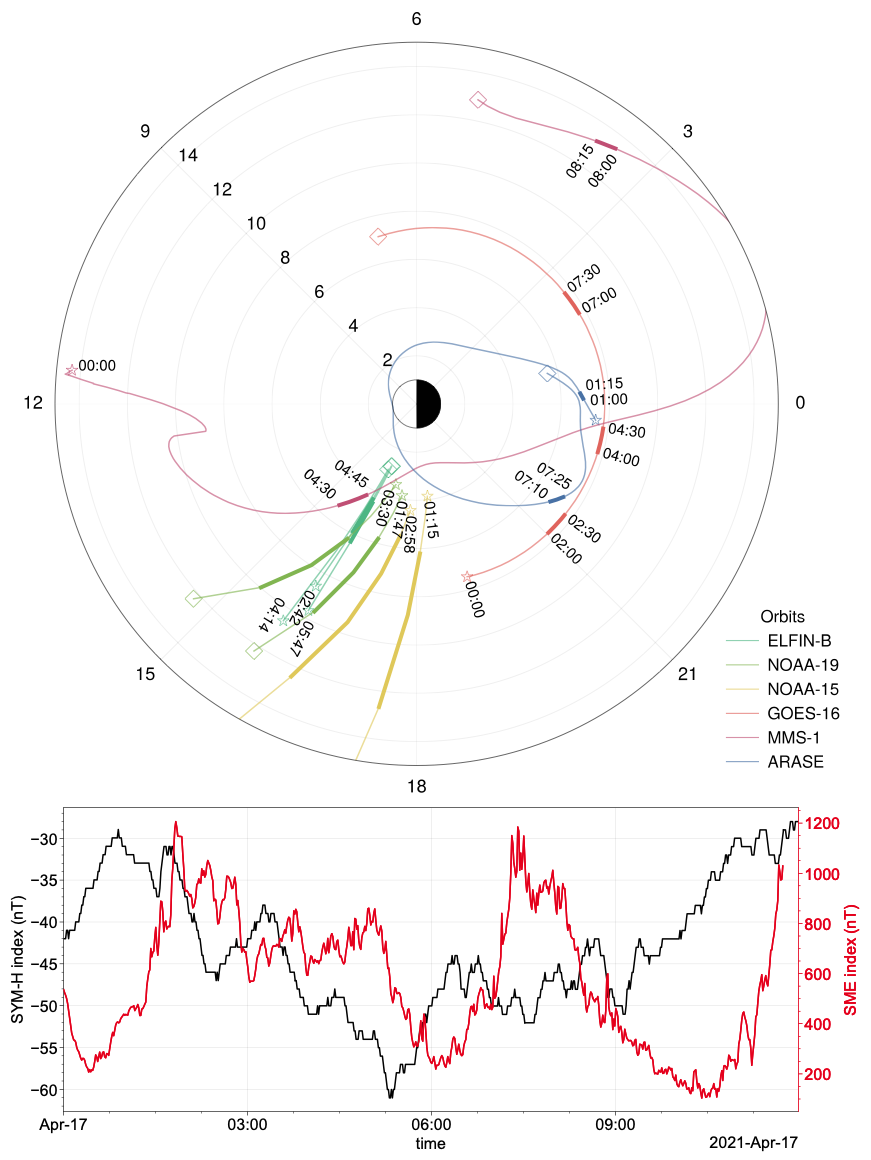
\includegraphics[width=0.67\textwidth,height=\textheight]{figures/fig1_orbit_multi_mission_conjunctions.png}

}

\caption{\label{fig-1}(top) An overview of the mission orbits recorded on April 17, 2021. The orbits of the various missions are projected onto the MLT and \(L\)-shell plane, using Tsyganenko model. (bottom) Sym-H and SME indices during this event.}

\end{figure}%

\subsection{Analysis Approach}\label{analysis-approach}

First, we will identify specific events during which intense EMIC wave activity coincides with significant changes in electron fluxes. These events will be used as case studies to analyze the interaction mechanisms in detail, employing cross-spectral analysis to examine the coherence between EMIC waves and electron flux oscillations.

\begin{figure}

\centering{

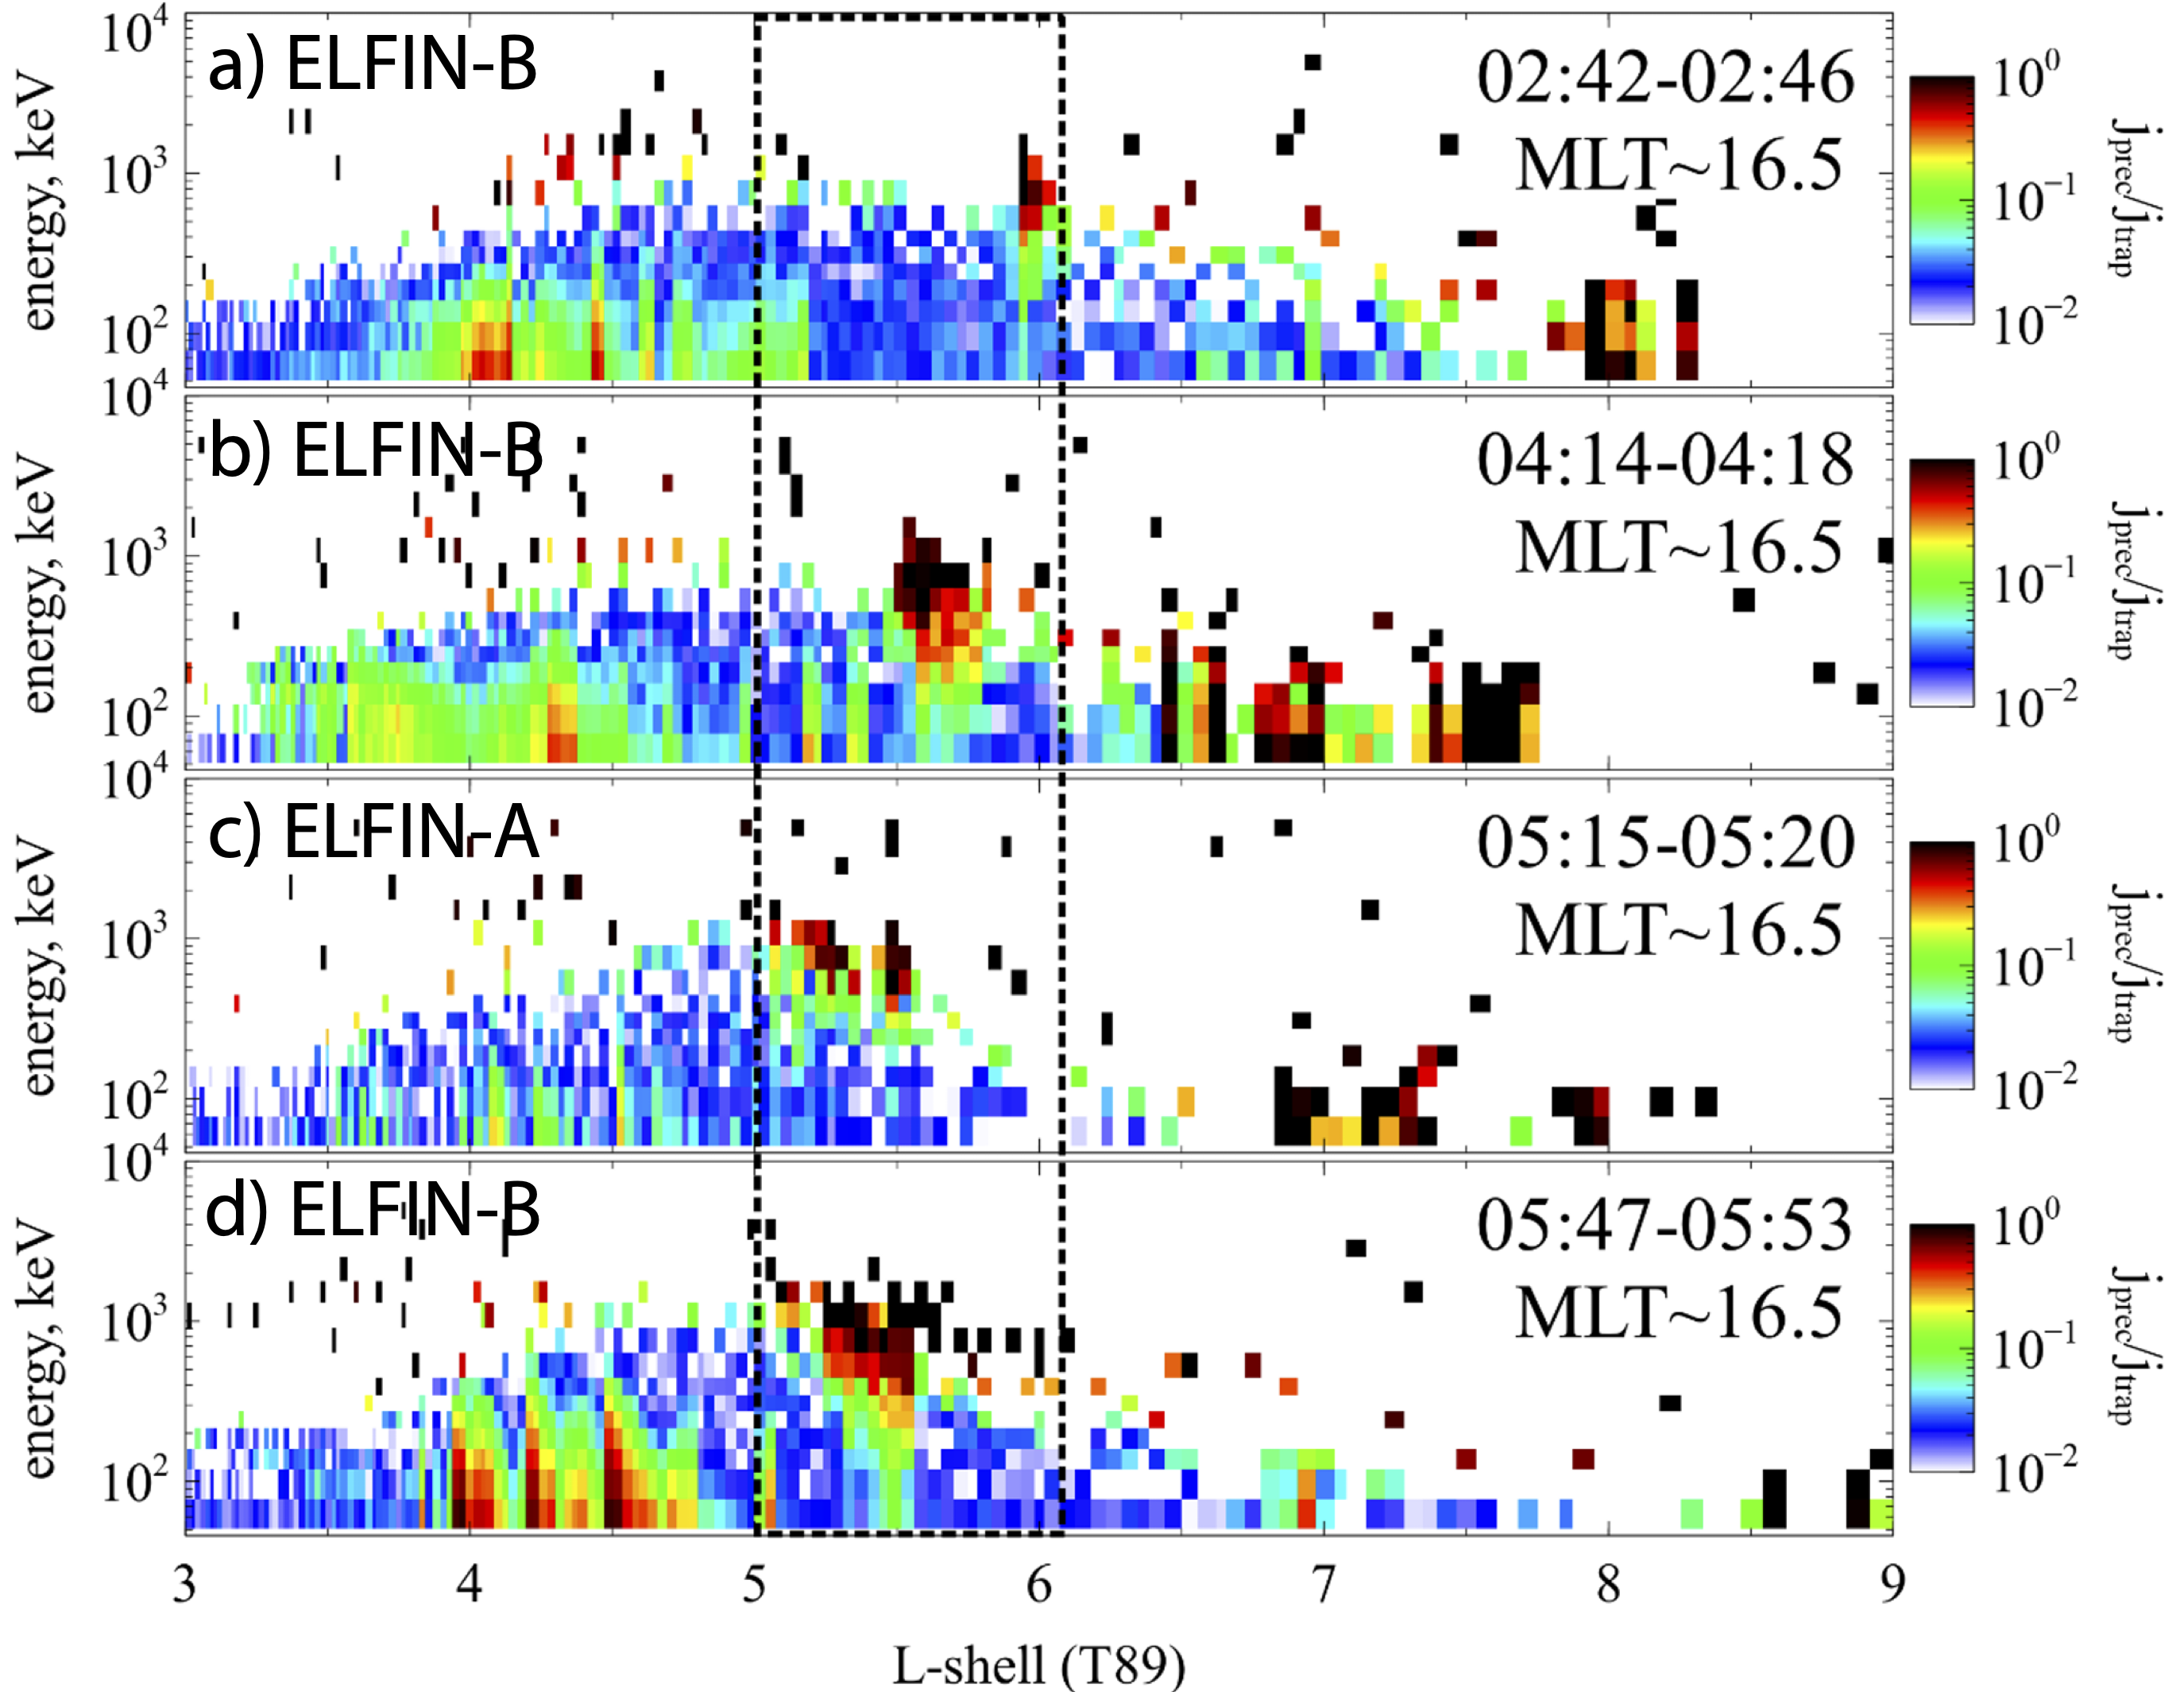
\includegraphics[width=0.67\textwidth,height=\textheight]{figures/fig_elfin_j_ratio.png}

}

\caption{\label{fig-elfin}Two ELFIN CubeSats observations of EMIC wave-driven electron precipitation, where the precipitating flux reaches the trapped flux in high-energy channels, over an interval exceeding three hours, from 02:42 to 05:53 UT. The locations are projected to the equatorial L-Shell and MLT, using the Tsyganenko89 magnetic field model. Panels (a), (b), and (d) show data from ELFIN-B, while panel (c) features observations from ELFIN-A.}

\end{figure}%

Figure~\ref{fig-elfin} (adapted from Fig 5 of \citet{angelopoulosEnergeticElectronPrecipitation2023}) shows a clear example of the EMIC wave-driven electron precipitation observed by ELFIN CubeSats. We observe a high precipitating-to-trapped flux ratio \(j_{prec}/j_{trap}\) during four ELFIN orbits.
Within \(L \in [5,6]\) there is a peak of precipitating-to-trapped flux ratio above \(300\) keV. This peak moves from \(L \sim 6\) around 02:45 UT to \(L \sim 5\) at 05:15 UT. Only EMIC wave-driven precipitation may have a low-energy cut-off of scattering fluxes around \(\sim 500\) keV, which is a typical minimum resonance energy for EMIC waves \citep[see the identification of other EMIC wave-driven precipitation events with similar precipitating-to-trapped ratios in][]{anNonresonantScatteringRelativistic2022, angelopoulosEnergeticElectronPrecipitation2023}. Note that the efficient precipitation (large \(j_{prec}/j_{trap}\)) observed at \(L>6.5\) is likely due to a combination of whistler-mode wave-driven precipitation \citep{shiRoleULFWaves2022} and precipitation due to the curvature scattering \citep{wilkinsStatisticalCharacteristicsElectron2023}, while precipitation of \(<300\) keV electrons at \(L<5\) is driven by whistler-mode wave scattering \citep[see similar examples of quasi-periodical precipitation on the dusk flank in][]{artemyevRoleDuctingRelativistic2021}.
Therefore, Figure~\ref{fig-elfin} demonstrates that during at least three hours, ELFIN observed continuous EMIC wave-driven losses of relativistic electrons. As \(j_{prec}/j_{trap}\) for \(\sim\) 0.3--1 MeV electrons reaches one, the strong diffusion regime, one may expect a significant depletion of equatorial electron flux in this energy range, at least at low pitch-angles.

To further confirm the role of EMIC waves in driving electron precipitation, we will utilize phase space density calculations and quasi-linear theory to analyze how EMIC waves scatter radiation belt electrons into the loss cone, leading to precipitation. By quantifying the diffusion coefficients, we can better understand the rate and extent of changes in electron flux.

In the limit of near-equilibrium of the electron distribution near the loss-cone \citep{kennelLimitStablyTrapped1966} the average precipitating electron flux measured within the loss-cone by ELFIN CubeSats at low altitude, \(j_{prec}\), can be expressed as a function of the trapped flux measured at an equatorial pitch-angle \(5\)\% above the loss-cone angle \(\alpha_{LC}\), denoted \(j_{trap}\) \citep{mourenasUpperLimitOuter2023}. In the ELFIN data products, \(j_{prec}\) is averaged over the loss cone weighted by solid angle, giving \(j_{prec}/j_{trap}\approx 1.3/(z_0+z_0^2/200)\) with \(z_0=2\alpha_{LC}/(\tau_B D_{\alpha\alpha})^{1/2}\) and \(\tau_B\) the electron bounce period, valid for \(j_{prec}/j_{trap}\in[0.001,0.85]\).
Accordingly, \(D_{\alpha\alpha}\) at \(\alpha_0=\alpha_{LC}\) can be inferred from the measured ratio \(j_{prec}/j_{trap}\) at ELFIN, giving \(D_{\alpha\alpha} \approx \frac{{\alpha_{LC}^2}}{{2500\, \tau_B }} \left(\sqrt{1+ \frac{{ j_{trap} }}{{ 38.5\, j_{prec} }} } -1 \right)^{-2}\).
The diffusion rates \(D_{\alpha\alpha}\) inferred, using the above Equation, from time-averaged ELFIN measurements of precipitating and trapped electron fluxes are displayed in Figure~\ref{fig-Daa_EMIC} for different electron energies and different \(L\). In the noon-dusk sector of the plasmaspheric plume, despite the theoretical impossibility of cyclotron resonance between 0.5-2 MeV electrons and typical EMIC wave frequencies, observed electron precipitation at these energies continues, particularly for low-energy electrons via scattering with high-frequency, low-amplitude H-band EMIC waves.
These results suggest the presence of duskside EMIC wave bursts with peak amplitudes \(B_w\approx 0.5\) nT and a low-amplitude component at frequencies above those of peak-amplitude.

This estimate of electron lifetime by EMIC waves is based on analytical quasi-linear diffusion theory with realistic wave and plasma parameters, which allows us to simplify the dispersion relation and the diffusion coefficients. However, in general, quasi-linear diffusion by EMIC waves alone cannot lead to strong and fast dropouts of 2--6 MeV electrons up to high pitch angles, as there is no cyclotron resonance between these electrons and EMIC waves above the maximum resonance pitch angle \(\alpha_{0,\max}\). This prevents the majority of the electron population from being scattered toward the loss cone, except if the bottleneck in the bounce-averaged pitch angle diffusion rate \(D_{\alpha\alpha}(\text{EMIC})\) at high \(\alpha_0\) can be filled by other kinds of waves. Therefore, in the proposed study, we will extend the quasi-linear diffusion analysis to chorus waves and further investigate the combined effects of EMIC and chorus waves on radiation belt electrons. By utilizing the observed wave properties with the aid of theoretical predictions, we aim to elucidate the underlying mechanisms that drive electron dynamics during storm-time events.

\subsection{Expected Contributions}\label{expected-contributions}

This project aims to quantify the impact of EMIC waves on the electron energy spectrum, previously thought to be shaped mainly by plasma injections and whistler-mode waves. Using data from satellite missions like ELFIN, Van Allen Probes, and ERG (Arase), we will examine how EMIC waves alter electron fluxes during storms, particularly alongside whistler-mode waves. By analyzing case studies and applying diffusion coefficients, we aim to assess how EMIC waves influence electron pitch angles and precipitation. Ultimately, this study seeks to compare the effects of EMIC and whistler-mode waves to determine when EMIC waves dominate electron loss processes.

\section{Discussion and Future Work}\label{discussion-and-future-work}

The findings of this research will deepen our comprehension of radiation belt electron dynamics in the presence of multiple waves during storm time. However, several questions are likely to arise from this study, guiding future research efforts:

\begin{itemize}
\item
  Wave Source Regions and Propagation: Further investigations may be required to identify the specific source regions of EMIC waves and their propagation characteristics through the magnetosphere. Understanding these aspects could enhance predictions of when and where EMIC waves will impact electron populations.
\item
  Interactions with Other Wave Modes: While this project focuses on EMIC waves, the magnetosphere contains multiple interacting wave modes. Future work could explore the interactions between EMIC waves and other wave types, such as ULF and VLF waves, to provide a more holistic view of the dynamics governing radiation belt electron fluxes.
\end{itemize}

\section{Summary}\label{summary}

The proposed research is designed to tackle some of the most pressing questions in space physics regarding the impact of EMIC\&whistler waves on radiation belt dynamics. Through a combination of detailed empirical analysis and advanced theoretical modeling, this project aims to provide significant insights and tools for predicting space weather, thereby contributing to our ability to safeguard and optimize the operation of space-based technologies.

\section{Figures}\label{figures}

\begin{figure}

\centering{

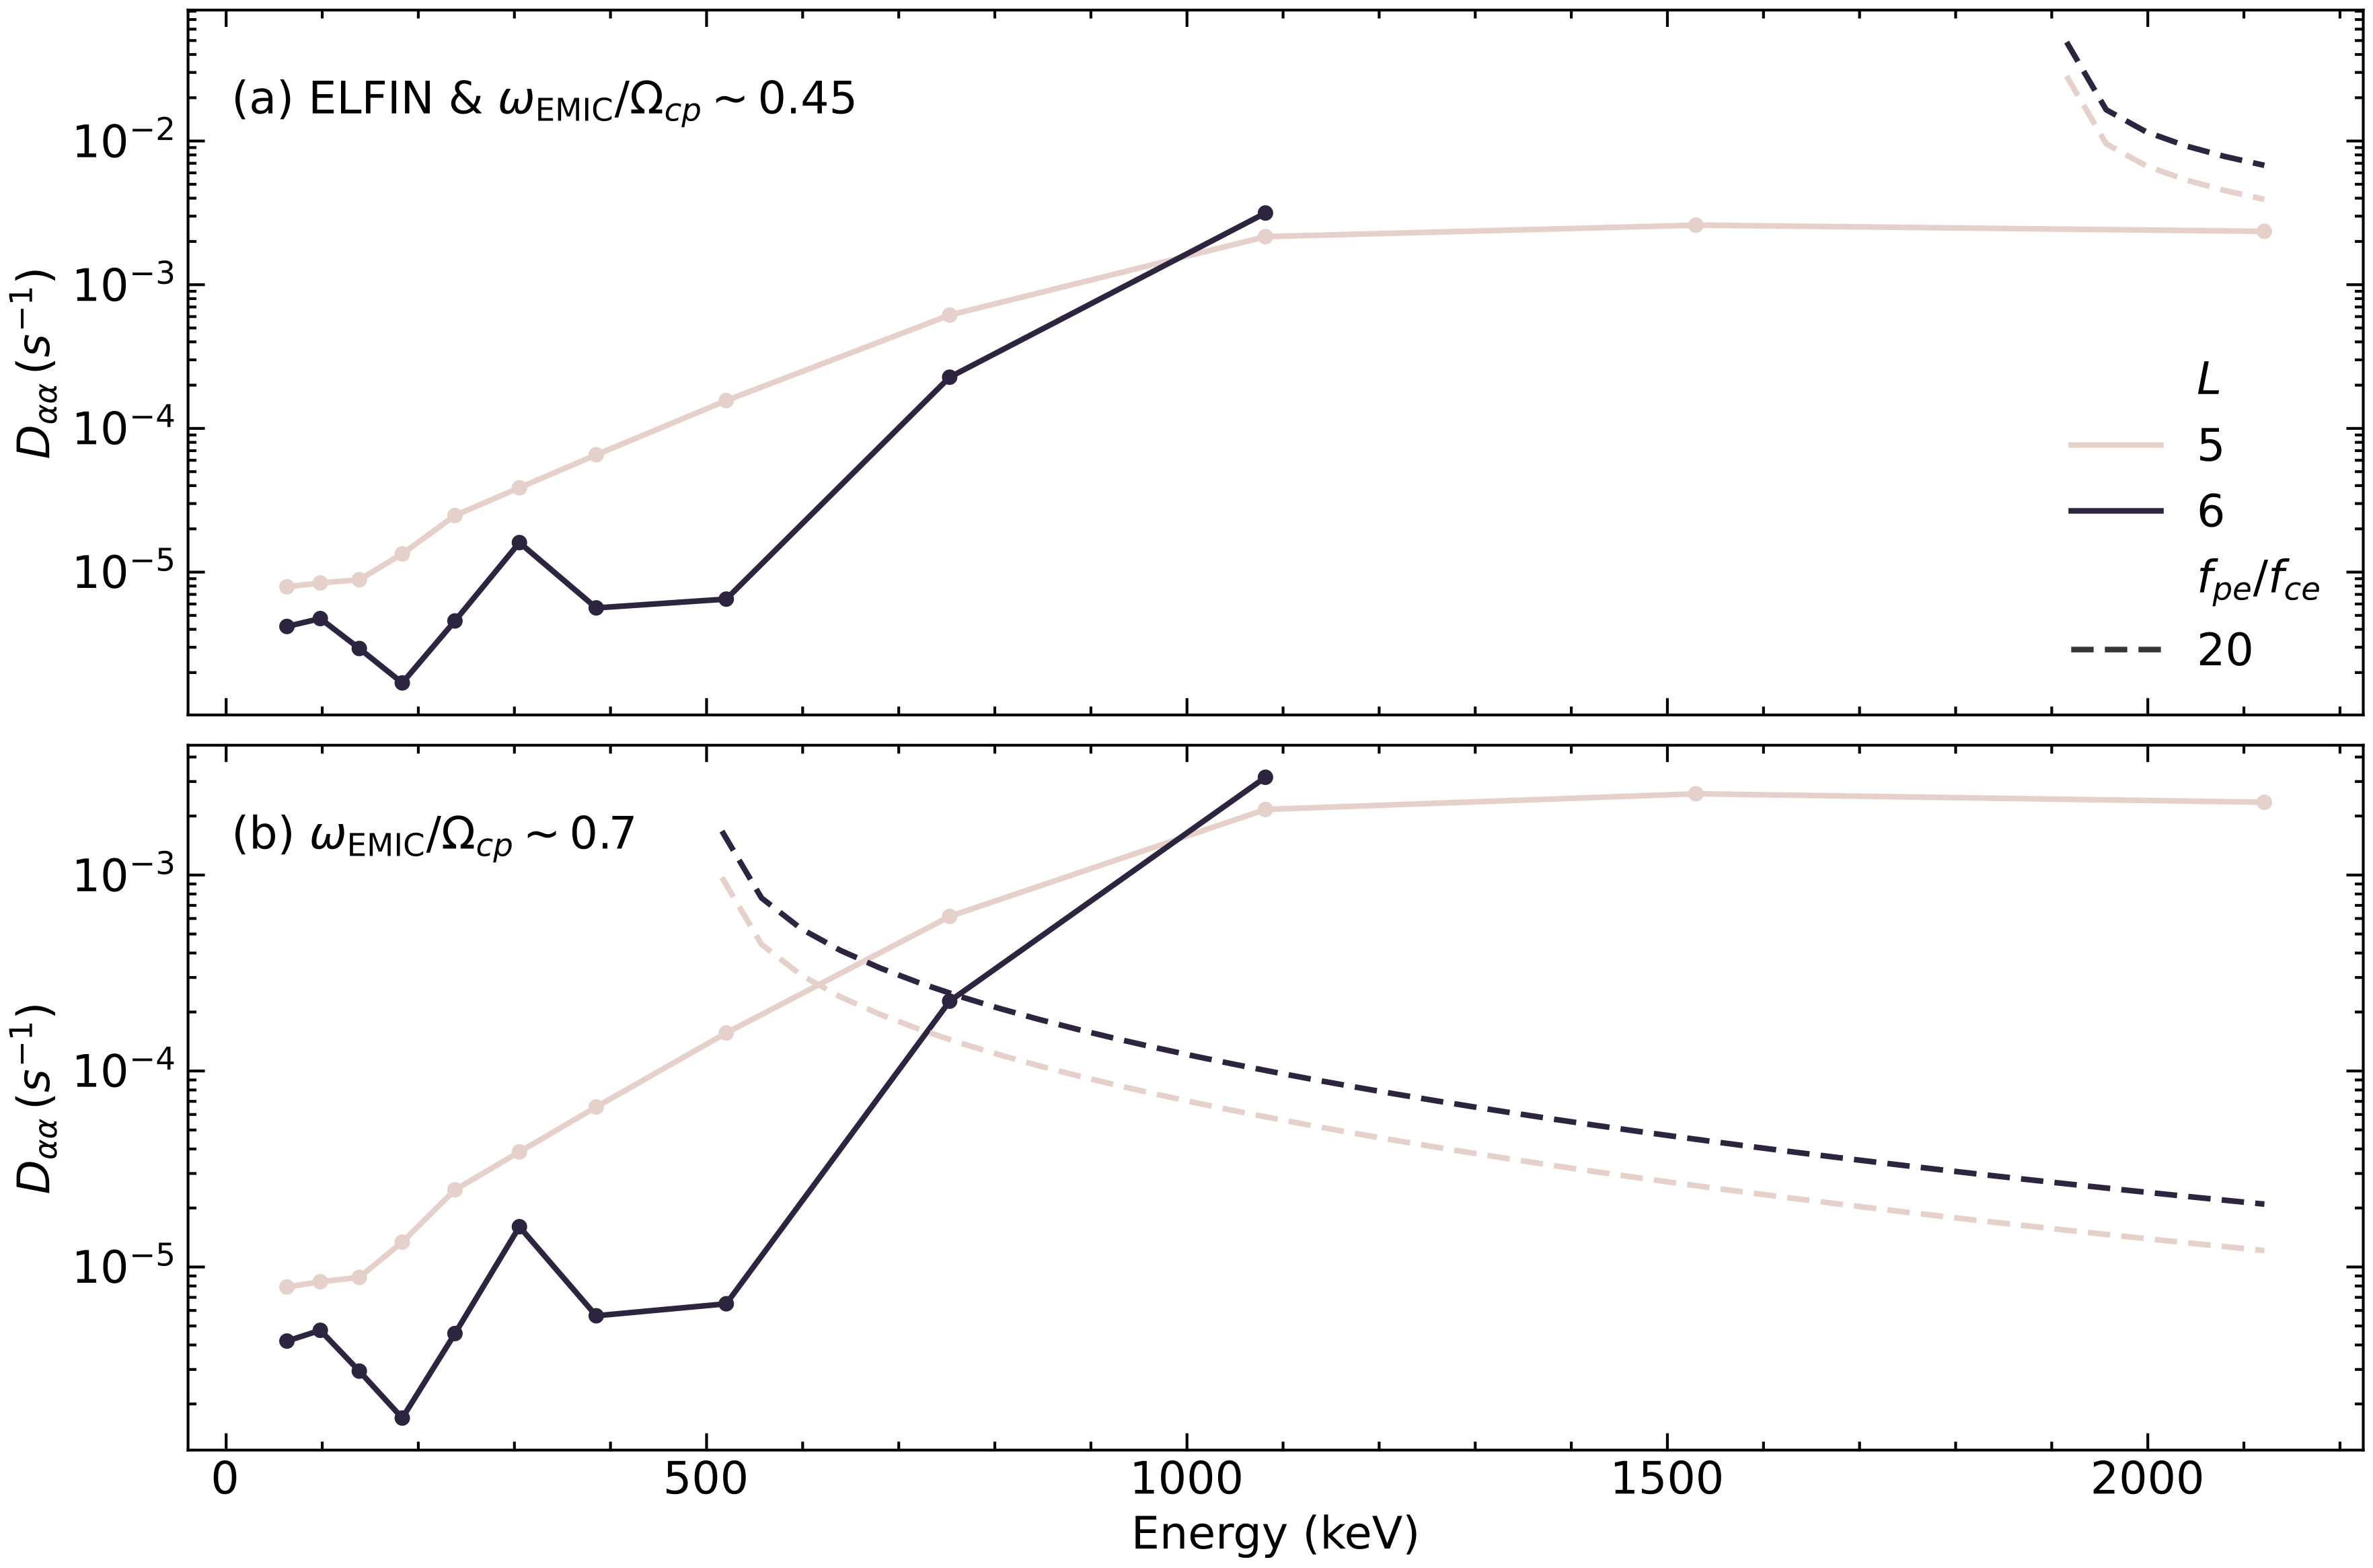
\includegraphics{figures/fig_Daa.png}

}

\caption{\label{fig-Daa_EMIC}Panel (a) Diffusion rates \(D_{\alpha\alpha}\) of electrons near the loss-cone inferred, using Equation 2, from ELFIN measurements of precipitating and trapped electron fluxes in the dusk sector near 16 MLT, at \(L=5\) (solid red) and \(L=6\) (solid black) as a function of electron energy \(E\). Diffusion rates \(D_{\alpha\alpha}\) near the loss-cone evaluated based on analytical estimates for H-band EMIC waves with typical wave and plasma parameters at \(L=5\) (red) and \(L=6\) (black) in a noon-dusk plasmaspheric plume, as a function of energy \(E\) are shown for a typical ratio \(f_{pe}/f_{ce}=20\), a peak wave amplitude of \(B_w=0.5\) nT at \(\omega_{\text{EMIC}}/\Omega_{cp}\sim 0.4\), and a (minimum) frequency \(\omega_{\text{EMIC}}/\Omega_{cp}\sim 0.45\) for cyclotron resonance with \(\sim2\) MeV electrons (dashed lines). (b) Same as (a) with analytical estimates of \(D_{\alpha\alpha}\) shown for H-band EMIC waves with a peak wave amplitude of \(B_w=0.5\) nT at \(\omega_{\text{EMIC}}/\Omega_{cp}\sim 0.4\) and a (minimum) frequency \(\omega_{\text{EMIC}}/\Omega_{cp}\sim 0.7\) for cyclotron resonance with \(\sim0.75\) MeV electrons (dashed lines).}

\end{figure}%

\newpage{}




\bibliography{files/Anton.addon.bib,files/Anton.full.bib,files/research.bib}


\end{document}
